% ----------------------------------------------------------
% MODELAGEM E DEFINIÇÕES TÉCNICAS
% ----------------------------------------------------------
\section{Modelagem e definições técnicas}
Esta seção tem por objetivo demonstrar as modelagens e padronizações utilizadas no desenvolvimento da aplicação.

\subsection{Modelo Entidade Relacionamento}

\begin{figure}[H]
	\centering 
	\caption{\label{fig:mer}Modelagem Entidade Relacionamento}
	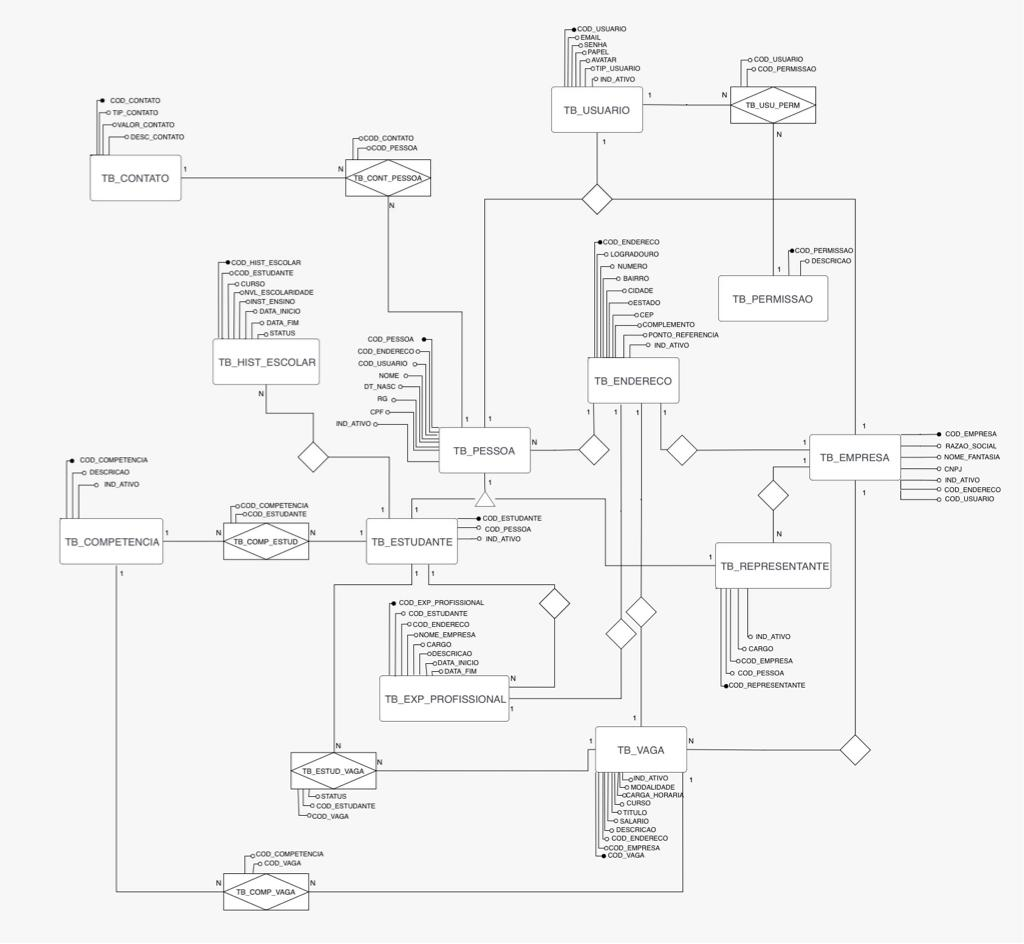
\includegraphics[width=\textwidth]{../imagens/mer-estagiei-3.jpeg} 
	\fonte{Os Autores}
\end{figure}

\subsection{Diagrama Entidade-Relacionamento}

\begin{figure}[H]
	\centering 
	\caption{\label{fig:der}Diagrama Entidade Relacionamento}
	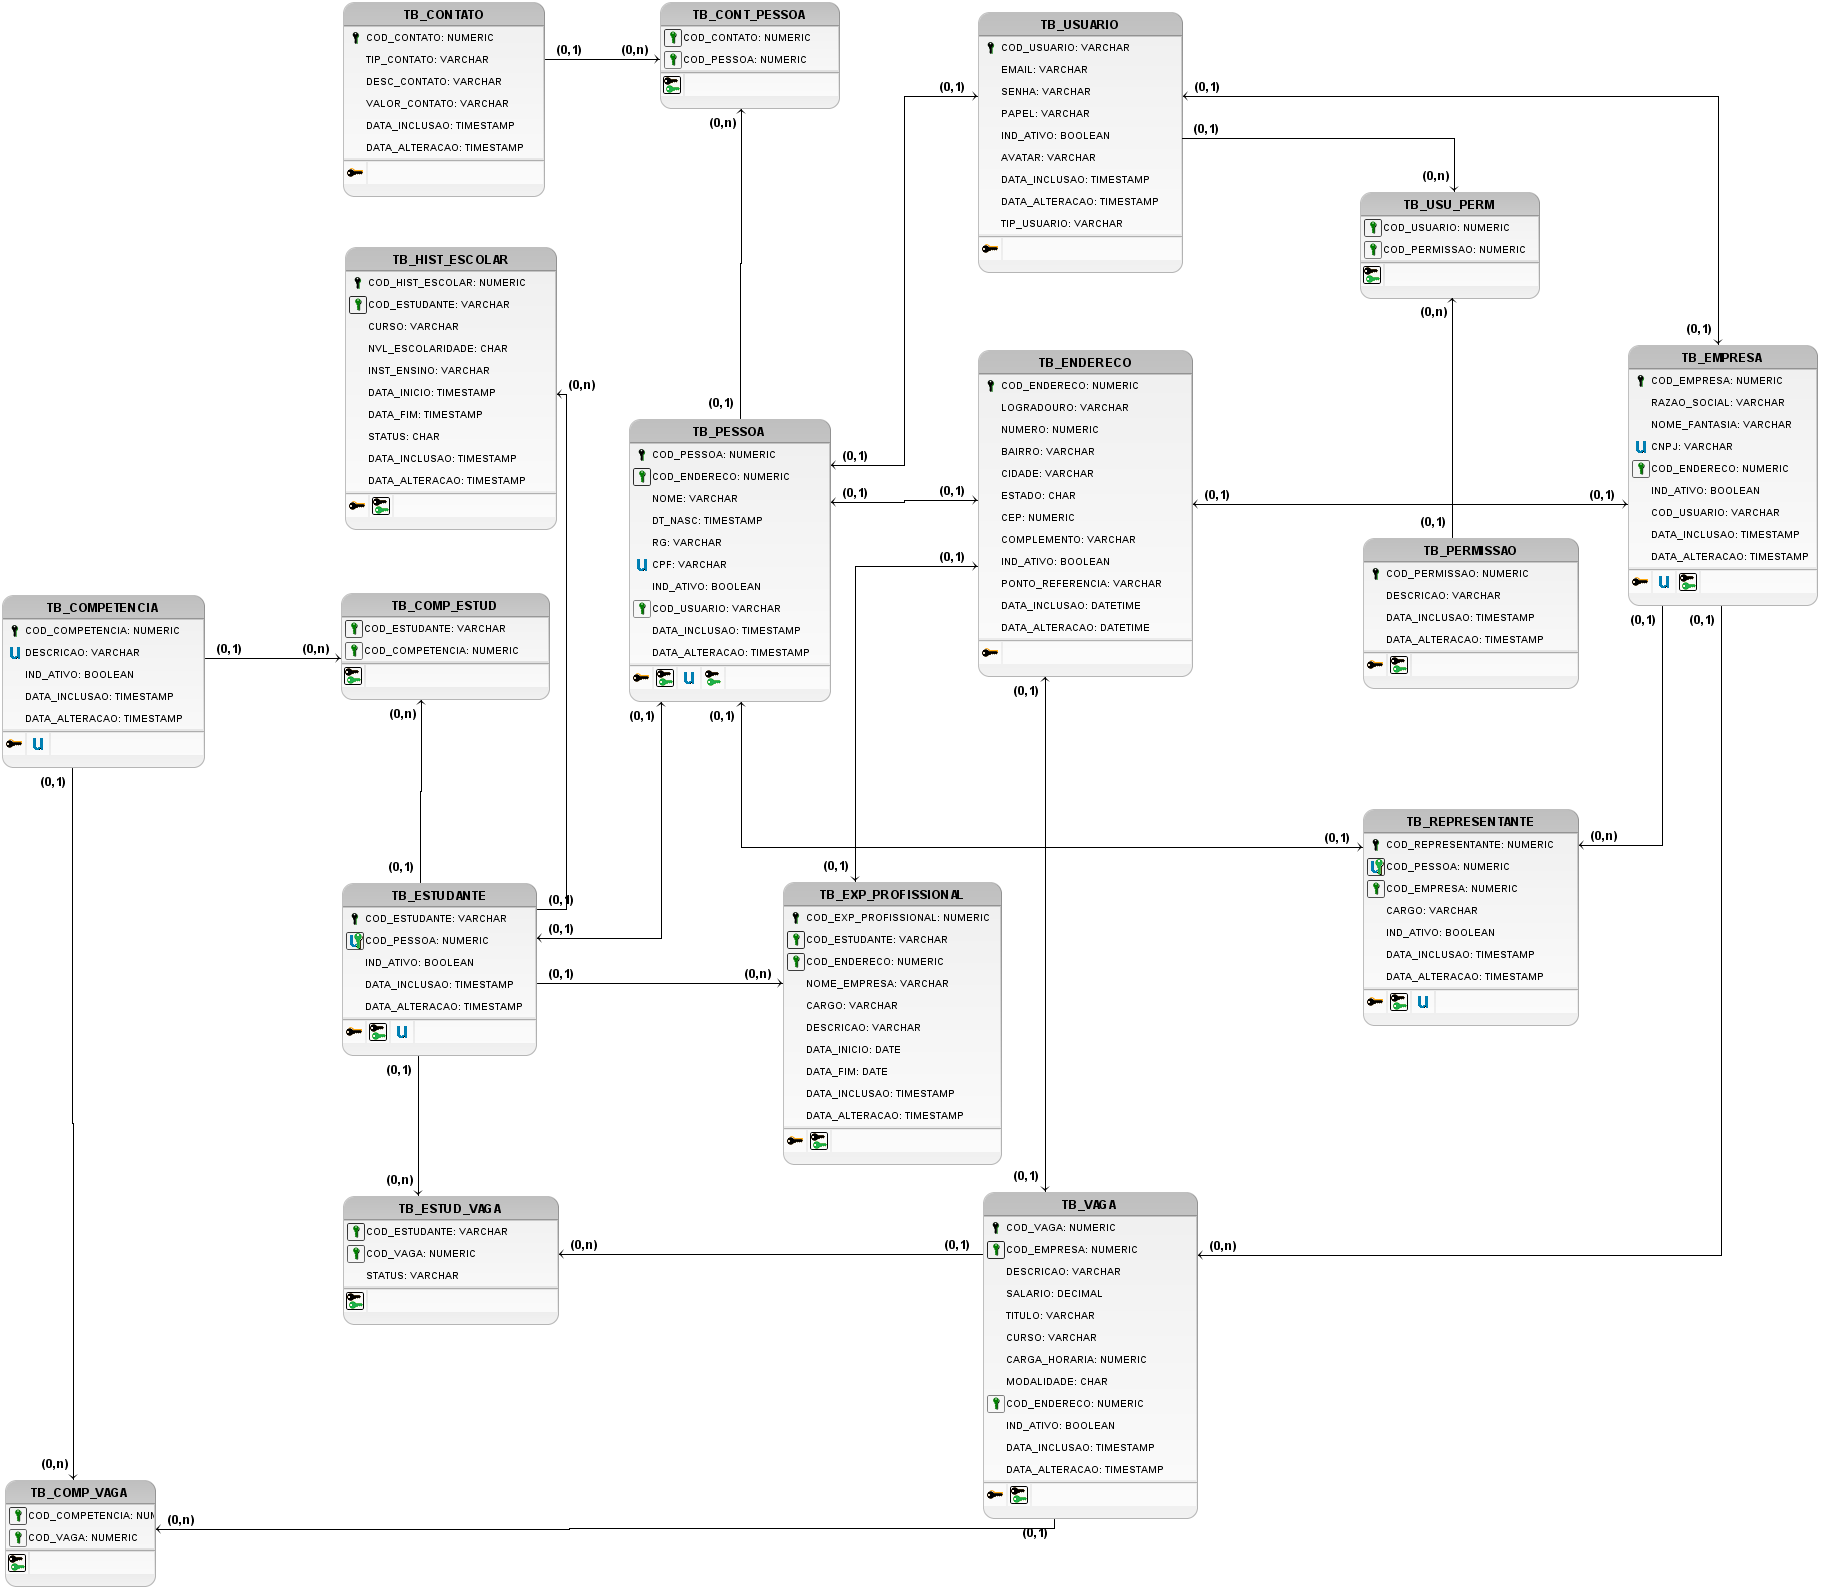
\includegraphics[width=\textwidth]{../imagens/der-estagiei-2.png} 
	\fonte{Os Autores}
\end{figure}

\subsection{Dicionário de Dados}
A seguir mostramos as tabelas do dicionário de dados. As tabelas de relacionamento foram omitidas.

\begin{quadro}[H]
	\caption{Legenda}
	\centering
	\begin{tabular}{| l | l |}
		\hline
		\thead{Sigla}	& \thead{Descrição}\\
		\hline
		PK			&   \textit{Primary Key}		\\
		\hline
		FK		    &  \textit{ Foregin Key}		\\
		\hline
		NN			&   \textit{Not Null}		\\
		\hline
		UQ			&   \textit{Unique}			\\
		\hline
		CK			&   \textit{Check}			\\
		\hline
		DEFAULT		&   \textit{Default}			\\
		\hline
	\end{tabular}
	\fonte{Os Autores}
	\label{legendas}
\end{quadro}

\begin{quadro}[H]
	\caption{Campos de Usuário}
	\centering
	\begin{tabular}{| l | l | l | p{0.3\textwidth} |}
		\hline
		\thead{Campo} & \thead{Tipo} & \thead{Restrição}	& \thead{Descrição}\\
		\hline
		Cod\_Usuario    & VARCHAR      & PK      & Identificador único para usuário         \\ 
		\hline
		Senha           & VARCHAR(50)  &         & Senha de acesso                          \\ 
		\hline
		Tip\_Usuario    & VARCHAR(3)   & NN &    Tipo do usuário no sistema    \\ 
		\hline
		E-mail          & VARCHAR(50)  &         & E-mail de acesso                          \\ 
		\hline
		Avatar          & VARCHAR(100) &         & Armazenamento de imagem do perfil \\ 
		\hline
		Ind\_Ativo      & BOOLEAN      & DEFAULT & Indicador de estado                      \\ 
		\hline
		Data\_Inclusao  & TIMESTAMP    &         & Campo auditável indicando data de inclusão        \\ 
		\hline
		Data\_Alteracao & TIMESTAMP    &         & Campo auditável indicando data de alteração                  \\ 
		\hline
	\end{tabular}
	\fonte{Os Autores}
	\label{campos-usuario}
\end{quadro}

\begin{quadro}[H]
	\caption{Campos de Pessoa}
	\centering
	\begin{tabular}{| l | l | l | p{0.3\textwidth} |}
		\hline
		\thead{Campo} & \thead{Tipo} & \thead{Restrição}	& \thead{Descrição}\\
		\hline
		Cod\_Pessoa   & SERIAL      & PK      & Identificador único para pessoa         \\ 
		\hline
		Cod\_Usuario  & SERIAL      & FK, NN  & Chave estrangeira vinda de tb\_usuario  \\
		\hline
		Cod\_Endereco & SERIAL      & FK, NN  & Chave estrangeira vinda de tb\_endereco \\ 
		\hline
		Nome          & VARCHAR(50) & NN      & Nome                                    \\ 
		\hline
		Dt\_Nasc      & DATE        & NN      & Data de nascimento                      \\ 
		\hline
		RG            & VARCHAR(11) & NN      & Registro Geral                          \\ 
		\hline
		CPF           & VARCHAR(13) & NN, UQ  & Cadastro de Pessoa Física               \\ 
		\hline
		Ind\_Ativo    & BOOLEAN     & DEFAULT & Indicador de estado                     \\ 
		\hline
		Data\_Inclusao  & TIMESTAMP &         & Campo auditável indicando data de inclusão        \\ 
		\hline
		Data\_Alteracao & TIMESTAMP &         & Campo auditável indicando data de alteração        \\ 
		\hline
	\end{tabular}
	\fonte{Os Autores}
	\label{campos-pessoa}
\end{quadro}

\begin{quadro}[H]
	\caption{Campos de Vaga}
	\centering
	\begin{tabular}{| l | l | l | p{0.3\textwidth} |}
		\hline
		\thead{Campo} & \thead{Tipo} & \thead{Restrição}	& \thead{Descrição}\\
		\hline
		Cod\_Vaga     & SERIAL      & PK      & Indicador único                 \\ 
		\hline
		Cod\_Empresa  & SERIAL      & FK NN   & Chave estrangeira de tb\_empresa  \\ 
		\hline
		Descricao     & TEXT        &         & Descrição da vaga                       \\ 
		\hline
		Salario       & FLOAT(5)    &         & Remuneração da vaga                     \\ 
		\hline
		Titulo        & VARCHAR(30) &         & Titulo da vaga                          \\ 
		\hline
		Curso         & VARCHAR(50) &         & Curso da vaga                          \\
		\hline
		Carga\_Horaria & INTEGER    & CK      & Carga horária da vaga                          \\
		\hline
		Modalidade     & CHAR       &         & Modalidade da vaga                          \\
		\hline   
		Cod\_Endereco & SERIAL      & FK NN   & Chave estrangeira de tb\_endereco \\ 
		\hline
		Ind\_Ativo    & BOOLEAN     & DEFAULT & Indicador de estado da vaga             \\ 
		\hline
		Data\_Inclusao  & TIMESTAMP &         & Campo auditável indicando data de inclusão        \\ 
		\hline
		Data\_Alteracao & TIMESTAMP &         & Campo auditável indicando data de alteração        \\ 
		\hline
	\end{tabular}
	\fonte{Os Autores}
	\label{campos-vaga}
\end{quadro}

\begin{quadro}[H]
	\caption{Campos de Estudante}
	\centering
	\begin{tabular}{| l | l | l | p{0.3\textwidth} |}
		\hline
		\thead{Campo} & \thead{Tipo} & \thead{Restrição}	& \thead{Descrição}\\
		\hline
		Cod\_Estudante         & VARCHAR      & PK          & Identificador único  \\ 
		\hline
		Cod\_Pessoa            & SERIAL       & FK, NN, UQ  & Chave estrangeira de tb\_pessoa            \\ 
		\hline
		Nvl\_Escolaridade      & VARCHAR(50)  &             & Nível de escolaridade do estudante     \\ 
		\hline
		Cod\_Exp\_Profissional & SERIAL       & FK          & Chave estrangeira  de tb\_exp\_profissional \\ 
		\hline
		Ind\_Ativo             & BOOLEAN      & DEFAULT     & Indicador de estado do estudante            \\ 
		\hline
		Data\_Inclusao         & TIMESTAMP    &             & Campo auditável indicando data de inclusão        \\ 
		\hline
		Data\_Alteracao        & TIMESTAMP    &             & Campo auditável indicando data de alteração        \\ 
		\hline
	\end{tabular}
	\fonte{Os Autores}
	\label{campos-estudante}
\end{quadro}

\begin{quadro}[H]
	\caption{Campos de Empresa}
	\centering
	\begin{tabular}{| l | l | l | p{0.3\textwidth} |}
		\hline
		\thead{Campo} & \thead{Tipo} & \thead{Restrição}	& \thead{Descrição}\\
		\hline
		Cod\_Empresa    & SERIAL      & PK      & Identificador único para a empresa      \\ 
		\hline
		Cod\_Usuario    & SERIAL      & FK, NN  & Chave estrangeira vinda de tb\_usuario  \\
		\hline
		Razao\_Social   & VARCHAR(50) & NN      & Razão social da empresa                 \\ 
		\hline
		Nome\_Fantasia  & VARCHAR(50) &         & Nome fantasia da empresa                \\ 
		\hline
		CNPJ            & VARCHAR(20) & NN, UQ  & Cadastro Nacional de Pessoas Jurídicas  \\ 
		\hline
		Cod\_Endereco   & SERIAL      & FK, NN  & Chave estrangeira vinda de tb\_endereco \\ 
		\hline
		Ind\_Ativo      & BOOLEAN     & DEFAULT & Indicador de estado da empresa          \\ 
		\hline
		Data\_Inclusao  & TIMESTAMP   &         & Campo auditável indicando data de inclusão        \\ 
		\hline
		Data\_Alteracao & TIMESTAMP   &         & Campo auditável indicando data de alteração        \\ 
		\hline
	\end{tabular}
	\fonte{Os Autores}
	\label{campos-empresa}
\end{quadro}

\begin{quadro}[H]
	\caption{Campos de Representante}
	\centering
	\begin{tabular}{| l | l | l | p{0.3\textwidth} |}
		\hline
		\thead{Campo} & \thead{Tipo} & \thead{Restrição}	& \thead{Descrição}\\
		\hline
		Cod\_Representante & SERIAL      & PK      & Identificador único                \\ 
		\hline
		Cod\_Pessoa        & SERIAL      & FK, NN  & Chave estrangeira de tb\_pessoa    \\ 
		\hline
		Cod\_Empresa       & SERIAL      & FK      & Chave estrangeira de tb\_empresa   \\ 
		\hline
		Cargo              & VARCHAR(50) & NN      & Descrição do cargo do representante \\ 
		\hline
		Ind\_Ativo         & BOOLEAN     & DEFAULT & Indicador de estado do representante   \\ 
		\hline
		Data\_Inclusao     & TIMESTAMP   &         & Campo auditável indicando data de inclusão        \\ 
		\hline
		Data\_Alteracao    & TIMESTAMP   &         & Campo auditável indicando data de alteração        \\ 
		\hline
	\end{tabular}
	\fonte{Os Autores}
	\label{campos-rh}
\end{quadro}

\begin{quadro}[H]
	\caption{Campos de Endereço}
	\centering
	\begin{tabular}{| l | l | l | p{0.3\textwidth} |}
		\hline
		\thead{Campo} & \thead{Tipo} & \thead{Restrição}	& \thead{Descrição}\\
		\hline
		Cod\_Endereco    & SERIAL      & PK      & Identificador único                \\ 
		\hline
		Logradouro        & VARCHAR(50)      & NN      & Logradouro do endereço    \\ 
		\hline
		Numero            & SMALLINT         &         & Número do endereço \\ 
		\hline
		Bairro            & VARCHAR(50)      & NN      & Bairro do endereço \\ 
		\hline
		Cidade            & VARCHAR(50)      & NN      & Cidade do endereço   \\ 
		\hline
		Estado            & CHAR(2)          & NN      & Estado do endereço \\ 
		\hline
		Cep               & CHAR(9)          &         & CEP do endereço \\ 
		\hline
		Complemento       & VARCHAR(50)      &         & Complemento do endereço \\ 
		\hline
		Ponto\_Referencia & VARCHAR(50)      &         & Ponto de referência do endereço \\ 
		\hline
		Ind\_Ativo        & BOOLEAN          & DEFAULT & Indicador de estado do endereço   \\ 
		\hline
		Data\_Inclusao    & TIMESTAMP        &         & Campo auditável indicando data de inclusão        \\ 
		\hline
		Data\_Alteracao   & TIMESTAMP        &         & Campo auditável indicando data de alteração        \\ 
		\hline
	\end{tabular}
	\fonte{Os Autores}
	\label{campos-rh}
\end{quadro}

\begin{quadro}[H]
	\caption{Campos de Competência}
	\centering
	\begin{tabular}{| l | l | l | p{0.3\textwidth} |}
		\hline
		\thead{Campo} & \thead{Tipo} & \thead{Restrição}	& \thead{Descrição}\\
		\hline
		Cod\_Competencia & SERIAL      & PK      & Identificador único                \\ 
		\hline
		Descricao        & VARCHAR(50)      &    & Descrição da competência    \\ 
		\hline
		Ind\_Ativo         & BOOLEAN     & DEFAULT & Indicador de estado da competência   \\ 
		\hline
		Data\_Inclusao  & TIMESTAMP &         & Campo auditável indicando data de inclusão        \\ 
		\hline
		Data\_Alteracao & TIMESTAMP &         & Campo auditável indicando data de alteração        \\ 
		\hline
	\end{tabular}
	\fonte{Os Autores}
	\label{campos-rh}
\end{quadro}

\begin{quadro}[H]
	\caption{Campos de Contato}
	\centering
	\begin{tabular}{| l | l | l | p{0.3\textwidth} |}
		\hline
		\thead{Campo} & \thead{Tipo} & \thead{Restrição}	& \thead{Descrição}\\
		\hline
		Cod\_Contato  & SERIAL      & PK      & Identificador único                \\ 
		\hline
		Tip\_Contato        & VARCHAR(10)      & CK    & Tipo do contato    \\ 
		\hline
		Desc\_Contato       & VARCHAR(50) & & Descrição do contato \\ 
		\hline
		Valor\_Contato & VARCHAR(100) &         & Valor do contato \\ 
		\hline
		Data\_Inclusao  & TIMESTAMP &         & Campo auditável indicando data de inclusão        \\ 
		\hline
		Data\_Alteracao & TIMESTAMP &         & Campo auditável indicando data de alteração        \\ 
		\hline
	\end{tabular}
	\fonte{Os Autores}
	\label{campos-rh}
\end{quadro}

\begin{quadro}[H]
	\caption{Campos de Experiência Profissional}
	\centering
	\begin{tabular}{| l | l | l | p{0.3\textwidth} |}
		\hline
		\thead{Campo} & \thead{Tipo} & \thead{Restrição}	& \thead{Descrição}\\
		\hline
		Cod\_Exp\_Profissional  & SERIAL      & PK      & Identificador único                \\ 
		\hline
		Cod\_Estudante        & SERIAL      & FK, NN    & Chave estrangeira de tb\_estudante    \\ 
		\hline
		Cod\_Endereco  & SERIAL      & FK, NN  & Chave estrangeira vinda de tb\_endereco \\ 
		\hline
		Nome\_Empresa & VARCHAR(100) &         & Nome da empresa da experiência \\ 
		\hline
		Cargo  & VARCHAR(75) &         & Cargo da experiência \\ 
		\hline
		Descricao  & TEXT &         & Breve descrição da experiência \\
		\hline
		Data\_Inicio  & TIMESTAMP &         & Data de início da experiência \\
		\hline
		Data\_Fim  & TIMESTAMP &         & Data de fim da experiência \\
		\hline
		Data\_Inclusao  & TIMESTAMP &         & Campo auditável indicando data de inclusão        \\ 
		\hline
		Data\_Alteracao & TIMESTAMP &         & Campo auditável indicando data de alteração        \\ 
		\hline
	\end{tabular}
	\fonte{Os Autores}
	\label{campos-rh}
\end{quadro}

\begin{quadro}[H]
	\caption{Campos de Histórico Escolar}
	\centering
	\begin{tabular}{| l | l | l | p{0.3\textwidth} |}
		\hline
		\thead{Campo} & \thead{Tipo} & \thead{Restrição}	& \thead{Descrição}\\
		\hline
		Cod\_Hist\_Escolar & SERIAL      & PK      & Identificador único                \\ 
		\hline
		Cod\_Estudante        & SERIAL      & FK, NN    & Chave estrangeira de tb\_estudante    \\ 
		\hline
		Nvl\_Escolaridade        & VARCHAR(50)      & & Nìvel de escolaridade    \\ 
		\hline
		Curso  & VARCHAR(50 )& & Curso do histórico \\ 
		\hline
		Inst\_Ensino & VARCHAR(50) &         & Instituição de ensino do histórico \\ 
		\hline
		Data\_Inicio  & TIMESTAMP &         & Data de início do histórico \\
		\hline
		Data\_Fim  & TIMESTAMP &         & Data de fim do histórico \\
		\hline
		Status  & VARCHAR(50) &         & Status do histórico escolar \\
		\hline
		Data\_Inicio  & TIMESTAMP &         & Data de início da experiência \\
		\hline
		Data\_Fim  & TIMESTAMP &         & Data de fim da experiência \\
		\hline
		Ind\_Ativo         & BOOLEAN     & DEFAULT & Indicador de estado do histórico   \\ 
		\hline
		Data\_Inclusao  & TIMESTAMP &         & Campo auditável indicando data de inclusão        \\ 
		\hline
		Data\_Alteracao & TIMESTAMP &         & Campo auditável indicando data de alteração        \\ 
		\hline
	\end{tabular}
	\fonte{Os Autores}
	\label{campos-rh}
\end{quadro}


\subsection{\textit{Endpoints} da API}
A seguir são apresentados os \textit{\glspl{endpoint}} mapeados até o momento, com seus respectivos métodos de requisição \gls{http}.

\begin{quadro}[H]
	\caption{\textit{\Glspl{endpoint}} de Estudante}
	\centering
	\begin{tabular}{| l | l |}
		\hline
		\thead{Método}	& \thead{\textit{Endpoint}}			\\
		\hline
		GET				& /api/estudante/\{codEstudante\}	\\
		\hline
		PUT				& /api/estudante/\{codEstudante\}	\\
		\hline
		POST			& /api/loginEstudante				\\
		\hline
		GET				& /api/estudante				\\
		\hline
		GET				& /api/estudante/\{codEstudante\}/recomendacao	\\
		\hline
	\end{tabular}
	\fonte{Os Autores}
	\label{endpoints-estudante}
\end{quadro}

\begin{quadro}[H]
	\caption{\textit{\Glspl{endpoint}} de Vaga}
	\centering
	\begin{tabular}{| l | l |}
		\hline
		\thead{Método}	& \thead{\textit{Endpoint}}	\\
		\hline
		GET				& /api/vaga	\\
		\hline
		POST			& /api/vaga	\\
		\hline
		GET				& /api/estudante/\{codEstudante\}/recomendacao	\\
		\hline
	\end{tabular}
	\fonte{Os Autores}
	\label{endpoints-vaga}
\end{quadro}


\begin{quadro}[H]
	\caption{\textit{\Glspl{endpoint}} de Empresa}
	\centering
	\begin{tabular}{| l | l |}
		\hline
		\thead{Método}	& \thead{\textit{Endpoint}}	\\
		\hline
		GET				& /api/empresa	\\
		\hline
		POST			& /api/empresa	\\
		\hline
		GET				& /api/empresa/\{codEmpresa\} \\
		\hline
	\end{tabular}
	\fonte{Os Autores}
	\label{endpoints-empresa}
\end{quadro}

\begin{quadro}[H]
	\caption{\textit{\Glspl{endpoint}} de Competência}
	\centering
	\begin{tabular}{| l | l |}
		\hline
		\thead{Método}	& \thead{\textit{Endpoint}}	\\
		\hline
		GET				& /api/competencia	\\
		\hline
	\end{tabular}
	\fonte{Os Autores}
	\label{endpoints-competencia}
\end{quadro}

\subsection{Listagem das Competências}
A seguir são apresentadas as competências parametrizadas a fim de realizar as recomendações de vagas para os estudantes de acordo com seu perfil. Essa listagem foi feita a partir do próprio conhecimento da equipe e complementada com pesquisas sobre as principais \textit{soft skills} requeridas no mercado \cite{fia_softskills,vagas_softskills, alura_softskills}. 

\begin{itemize}
	\label{softskills}
	\item Adaptação
	\item Atitude positiva
	\item Autoconfiança
	\item Autogestão
	\item Boa escrita
	\item Capacidade de resolver problemas
	\item Capacidade de tomar decisões
	\item \textit{Coaching}
	\item Colaboração
	\item Comunicação
	\item Conhecimento político e cultural
	\item Criatividade
	\item Desenvolvimento da esquipe
	\item Desenvolvimento pessoal
	\item Empatia
	\item Estabelecimento de confiança
	\item Ética no trabalho
	\item Flexibilidade
	\item Gerenciamento de conflitos
	\item Honestidade
	\item Influência
	\item Inteligência emocional
	\item Interesse em aprender
	\item Liderança
	\item Motivação
	\item Organização
	\item Pensamento crítico
	\item Poder de negociação
	\item Proatividade
	\item Relacionamento interpessoal
	\item Resiliência
	\item Trabalho em Equipe
	\item Trabalho sob pressão
\end{itemize}